% =====================================================================
%  Capítulo 2. Hechos estilizados de los rendimientos financieros
% =====================================================================
\chapter{Hechos estilizados de los rendimientos financieros}\label{cap:hechos}

\section*{Objetivos de aprendizaje}
Al terminar este capítulo, el lector podrá:
\begin{enumerate}[label=\arabic*.,leftmargin=*]
  \item Calcular e interpretar la asimetría y la curtosis muestrales, y derivar su distribución asintótica
        bajo normalidad.
  \item Demostrar y aplicar la prueba de Jarque-Bera, y explicar por qué rechaza casi siempre con datos
        financieros diarios.
  \item Medir el grosor de las colas con el índice de Hill y relacionarlo con la existencia de momentos.
  \item Distinguir entre ausencia de autocorrelación e independencia, usando la autocorrelación de los
        rendimientos, de sus cuadrados y de sus valores absolutos.
  \item Reconocer los artefactos que crean los datos promediados (efecto de Working).
  \item Enunciar los hechos estilizados que los modelos de los capítulos siguientes deben reproducir.
\end{enumerate}

\section*{Motivación}
El 21 de abril de 2020, en plena paralización mundial por la pandemia, el precio spot del petróleo Brent
cayó de 17,36 a 9,12 dólares por barril: un rendimiento logarítmico de $-64$\,\% en un solo día. Al día
siguiente subió 41\,\%. Si los rendimientos diarios del Brent fueran normales, con la volatilidad que
muestran sus casi cuatro décadas de historia, una caída así sería un suceso de 24 desviaciones estándar:
algo que no debería ocurrir ni una sola vez en la vida del universo. Ocurrió, y no fue el único: la
historia del Brent tiene 51 días con movimientos mayores a cuatro desviaciones estándar, cuando la
normal predice menos de uno.

Este capítulo documenta, con datos reales, las regularidades empíricas que comparten los rendimientos de
casi todos los activos financieros: los \emph{hechos estilizados}. No son curiosidades: determinan qué
modelos tienen sentido, qué pruebas estadísticas son válidas y cuánto riesgo se subestima al suponer
normalidad. Cada hecho que documentemos aquí será, más adelante, la motivación de un modelo: el
agrupamiento de volatilidad lleva a los modelos GARCH (Capítulos~8 y~9) y las colas pesadas, a la teoría
de valores extremos del valor en riesgo (Capítulo~13).

\paragraph{Datos del capítulo.} Usamos tres series reales, descargadas el 6 de noviembre de 2026 de los
repositorios públicos \texttt{datasets} de GitHub, que replican automáticamente las fuentes oficiales:
\begin{itemize}[leftmargin=*]
  \item \textbf{Petróleo Brent}, precio spot diario en dólares por barril, del 20 de mayo de 1987 al 3 de
        noviembre de 2026 (9\,122 precios). Fuente original: Administración de Información Energética de
        EE.\,UU. (EIA).
  \item \textbf{S\&P 500 mensual} de la base de datos de Robert Shiller, de enero de 1871 a septiembre de
        2026 (1\,869 precios). Cada dato es el \emph{promedio} de los cierres diarios del mes, un detalle
        decisivo en la Sección~\ref{sec:working}.
  \item \textbf{VIX}, índice de volatilidad de CBOE, diario, de 1990 a septiembre de 2026 (usado en los
        ejercicios propuestos).
\end{itemize}
Los archivos están en \texttt{datos/internacional/} junto con un registro de fuentes. Las aplicaciones
al mercado peruano (índice S\&P/BVL Perú General y acciones mineras) se plantean como ejercicios
propuestos con los datos del Capítulo~\ref{cap:rendimientos}.

% ---------------------------------------------------------------------
\section{Momentos muestrales y la prueba de Jarque-Bera}
% ---------------------------------------------------------------------

Sea $r_1,\dots,r_T$ una muestra de rendimientos logarítmicos, con media $\bar r=\frac1T\sum_tr_t$.

\begin{definicion}[Momentos muestrales centrados]
Para $j\ge 2$, el momento muestral centrado de orden $j$ es $m_j=\frac1T\sum_{t=1}^T(r_t-\bar r)^j$. La
\emph{desviación estándar}, la \emph{asimetría} y la \emph{curtosis} muestrales son
\[
  \hat\sigma=\sqrt{m_2},\qquad \hat S=\frac{m_3}{m_2^{3/2}},\qquad \hat K=\frac{m_4}{m_2^{2}} .
\]
\end{definicion}

La asimetría mide si las desviaciones grandes son más frecuentes de un lado que del otro; un valor
negativo indica que las caídas extremas son más intensas que las subidas extremas. La curtosis mide el
peso de las colas en relación con el centro: para la distribución normal $K=3$, y una curtosis mayor
indica \emph{leptocurtosis}: más observaciones cerca de la media y en las colas, y menos en los
hombros. A $K-3$ se le llama \emph{exceso de curtosis}. La Figura~\ref{fig:momentos} ilustra ambos conceptos con densidades que tienen la misma media y la misma varianza, para que lo único que cambie sea la forma.
\begin{figure}[ht]
\centering
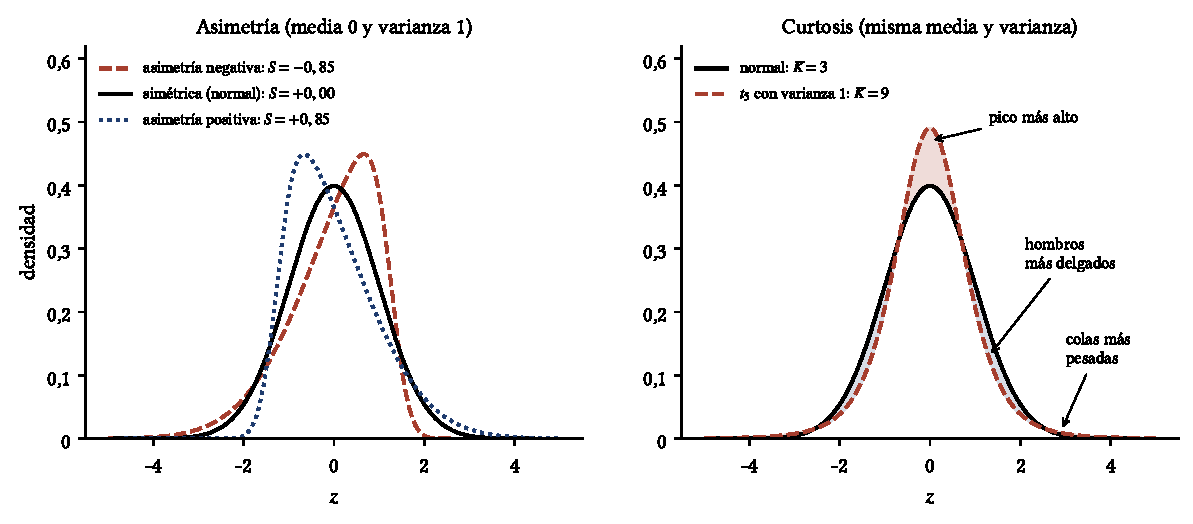
\includegraphics[width=\linewidth]{graficos/cap02_fig_momentos.pdf}
\caption{Izquierda: tres densidades con media 0 y varianza 1 (normal asimétrica). Con asimetría negativa la cola larga está a la izquierda: las caídas extremas son más probables que las subidas extremas. Derecha: normal frente a una $t_5$ reescalada a varianza 1. La $t_5$ tiene más masa en el centro y en las colas (sombreado rojo) y menos en los hombros (sombreado azul): eso es la leptocurtosis.}
\label{fig:momentos}
\end{figure}


\begin{observacion}
Usamos el divisor $T$ (no $T-1$) en todos los momentos, que es la convención de la prueba de Jarque-Bera
y la opción por defecto de \texttt{scipy.stats.skew} y \texttt{scipy.stats.kurtosis}. Otros programas
aplican correcciones de sesgo pequeño; con miles de datos la diferencia es despreciable, pero conviene
saber qué calcula cada función antes de comparar resultados.
\end{observacion}

\begin{teorema}[Distribución asintótica bajo normalidad]\label{teo:jb}
Si $r_1,\dots,r_T$ son independientes e idénticamente distribuidos (i.i.d.) con distribución
$N(\mu,\sigma^2)$, entonces, cuando $T\to\infty$,
\[
  \sqrt T\,\hat S\xrightarrow{d}N(0,6),\qquad \sqrt T\,(\hat K-3)\xrightarrow{d}N(0,24),
\]
y ambos estadísticos son asintóticamente independientes. En consecuencia, el estadístico de
\emph{Jarque-Bera}
\[
  JB=T\left[\frac{\hat S^2}{6}+\frac{(\hat K-3)^2}{24}\right]
\]
converge en distribución a una $\chi^2$ con 2 grados de libertad.
\end{teorema}

\begin{proof}
Como $\hat S$ y $\hat K$ no cambian si los datos se trasladan o se reescalan, basta con considerar
$z_t=(r_t-\mu)/\sigma\sim N(0,1)$. Usaremos los momentos de la normal estándar:
\[
  \E z=\E z^3=\E z^5=\E z^7=0,\qquad \E z^2=1,\qquad \E z^4=3,\qquad \E z^6=15,\qquad \E z^8=105 .
\]
Escribimos $\overline{g}=\frac1T\sum_tg(z_t)$ para cualquier función $g$. Por la ley de los grandes números
$\overline{g}\to\E g(z)$, y por el teorema central del límite $\bar z=O_p(T^{-1/2})$ y
$\overline{z^3}=O_p(T^{-1/2})$.

\emph{Paso 1: asimetría.} Desarrollando el cubo y promediando:
\begin{align*}
  m_3 &= \frac1T\sum_t(z_t-\bar z)^3\\
      &= \overline{z^3}-3\bar z\,\overline{z^2}+3\bar z^2\,\bar z-\bar z^3\\
      &= \overline{z^3}-3\bar z\,\overline{z^2}+2\bar z^3.
\end{align*}
Multiplicando por $\sqrt T$ y usando $\overline{z^2}=1+o_p(1)$ y $\bar z^3=O_p(T^{-3/2})$:
\begin{align*}
  \sqrt T\,m_3 &= \sqrt T\,\overline{z^3}-3\sqrt T\,\bar z\,\overline{z^2}+2\sqrt T\,\bar z^3\\
               &= \sqrt T\,\overline{z^3}-3\sqrt T\,\bar z+o_p(1)\\
               &= \frac1{\sqrt T}\sum_{t=1}^T\bigl(z_t^3-3z_t\bigr)+o_p(1).
\end{align*}
Como $m_2\to1$, $\sqrt T\hat S=\sqrt T\,m_3/m_2^{3/2}$ tiene el mismo límite (teorema de Slutsky). La
variable $u_t=z_t^3-3z_t$ tiene media cero y varianza
\begin{align*}
  \E[u_t^2] &= \E\bigl[z^6-6z^4+9z^2\bigr]\\
            &= 15-6\cdot3+9\cdot1\\
            &= 6 .
\end{align*}
Por el teorema central del límite, $\sqrt T\hat S\xrightarrow{d}N(0,6)$.

\emph{Paso 2: curtosis.} Desarrollando la cuarta potencia y promediando:
\begin{align*}
  m_4 &= \overline{z^4}-4\bar z\,\overline{z^3}+6\bar z^2\,\overline{z^2}-3\bar z^4\\
      &= \overline{z^4}+O_p(T^{-1}),
\end{align*}
porque $\bar z\,\overline{z^3}$ y $\bar z^2$ son $O_p(T^{-1})$. Para el denominador:
\begin{align*}
  m_2      &= \overline{z^2}-\bar z^2\\
           &= 1+\overline{(z^2-1)}+O_p(T^{-1}),\\
  m_2^{-2} &= 1-2\,\overline{(z^2-1)}+O_p(T^{-1}).
\end{align*}
Multiplicando, y usando $\overline{z^4}=3+O_p(T^{-1/2})$ en el término cruzado:
\begin{align*}
  \hat K &= m_4\,m_2^{-2}\\
         &= \overline{z^4}\,\bigl(1-2\,\overline{(z^2-1)}\bigr)+O_p(T^{-1})\\
         &= \overline{z^4}-6\,\overline{(z^2-1)}+O_p(T^{-1})\\
         &= 3+\overline{(z^4-3)}-6\,\overline{(z^2-1)}+O_p(T^{-1}).
\end{align*}
Por tanto,
\begin{align*}
  \sqrt T(\hat K-3) &= \frac1{\sqrt T}\sum_{t=1}^T\bigl[(z_t^4-3)-6(z_t^2-1)\bigr]+o_p(1)\\
                    &= \frac1{\sqrt T}\sum_{t=1}^Tv_t+o_p(1), \qquad v_t=z_t^4-6z_t^2+3 .
\end{align*}
La variable $v_t$ tiene media $3-6+3=0$ y varianza
\begin{align*}
  \E[v_t^2] &= \E\bigl[z^8-12z^6+42z^4-36z^2+9\bigr]\\
            &= 105-12\cdot15+42\cdot3-36\cdot1+9\\
            &= 105-180+126-36+9\\
            &= 24 .
\end{align*}

\emph{Paso 3: independencia y Jarque-Bera.} La covarianza entre $u_t$ y $v_t$ solo contiene momentos
impares:
\begin{align*}
  \E[u_tv_t] &= \E\bigl[(z^3-3z)(z^4-6z^2+3)\bigr]\\
             &= \E\bigl[z^7-9z^5+21z^3-9z\bigr]\\
             &= 0 .
\end{align*}
Por el teorema central del límite multivariado, $\sqrt T(\hat S,\hat K-3)$ converge a una normal bivariada
con matriz de covarianzas $\operatorname{diag}(6,24)$. Los dos componentes estandarizados son normales
estándar independientes en el límite, y la suma de sus cuadrados es una $\chi^2_2$:
\begin{align*}
  JB &= \Bigl(\frac{\sqrt T\,\hat S}{\sqrt6}\Bigr)^2+\Bigl(\frac{\sqrt T\,(\hat K-3)}{\sqrt{24}}\Bigr)^2\\
     &= T\Bigl[\frac{\hat S^2}{6}+\frac{(\hat K-3)^2}{24}\Bigr]\\
     &\xrightarrow{d}\chi^2_2 . && \qedhere
\end{align*}
\end{proof}

\begin{observacion}[Lo que la prueba no dice]
Con $T$ grande, $JB$ rechaza la normalidad ante desviaciones minúsculas. En finanzas el rechazo es tan
seguro que el valor del estadístico importa menos que el diagnóstico: \emph{qué} momento falla y
\emph{por qué}. Además, el Teorema~\ref{teo:jb} supone observaciones independientes. Con datos
financieros, que presentan agrupamiento de volatilidad (Sección~\ref{sec:acf}), la distribución nula de
$JB$ deja de ser exactamente $\chi^2_2$ incluso cuando la distribución marginal fuera normal.
\end{observacion}

% ---------------------------------------------------------------------
\section{Colas pesadas}\label{sec:colas}
% ---------------------------------------------------------------------

\subsection{La distribución $t$ de Student}

La primera alternativa a la normal con colas más pesadas es la $t$ de Student, que usaremos en los
modelos GARCH del Capítulo~9.

\begin{proposicion}\label{prop:curt_t}
Si $X\sim t_\nu$ con $\nu>4$, entonces $\Var(X)=\nu/(\nu-2)$ y su curtosis es
\[
  K=3+\frac{6}{\nu-4}>3 .
\]
Para $\nu\le 4$ el cuarto momento no existe.
\end{proposicion}

\begin{proof}
Representamos $X=Z/\sqrt{W/\nu}$, con $Z\sim N(0,1)$ independiente de $W\sim\chi^2_\nu$. Por
independencia,
\begin{align*}
  \E[X^2] &= \nu\,\E[Z^2]\,\E[W^{-1}] = \nu\,\E[W^{-1}],\\
  \E[X^4] &= \nu^2\,\E[Z^4]\,\E[W^{-2}] = 3\nu^2\,\E[W^{-2}].
\end{align*}
Con la densidad de la $\chi^2_\nu$, $f(w)=w^{\nu/2-1}e^{-w/2}/\bigl(2^{\nu/2}\Gamma(\nu/2)\bigr)$:
\begin{align*}
  \E[W^{-m}] &= \int_0^\infty w^{-m}\,\frac{w^{\nu/2-1}e^{-w/2}}{2^{\nu/2}\Gamma(\nu/2)}\,dw\\
             &= \frac{1}{2^{\nu/2}\Gamma(\nu/2)}\int_0^\infty w^{(\nu/2-m)-1}e^{-w/2}\,dw\\
             &= \frac{2^{\nu/2-m}\,\Gamma(\nu/2-m)}{2^{\nu/2}\,\Gamma(\nu/2)}\\
             &= \frac{\Gamma(\nu/2-m)}{2^m\,\Gamma(\nu/2)},
\end{align*}
que es finita solo si $\nu/2-m>0$. Usando $\Gamma(a+1)=a\,\Gamma(a)$:
\begin{align*}
  \E[W^{-1}] &= \frac{\Gamma(\nu/2-1)}{2\,(\nu/2-1)\,\Gamma(\nu/2-1)} = \frac{1}{\nu-2},\\
  \E[W^{-2}] &= \frac{\Gamma(\nu/2-2)}{4\,(\nu/2-1)(\nu/2-2)\,\Gamma(\nu/2-2)} = \frac{1}{(\nu-2)(\nu-4)}.
\end{align*}
Entonces:
\begin{align*}
  \Var(X) &= \frac{\nu}{\nu-2},\\
  \E[X^4] &= \frac{3\nu^2}{(\nu-2)(\nu-4)},\\
  K       &= \frac{\E[X^4]}{(\Var X)^2}\\
          &= \frac{3\nu^2}{(\nu-2)(\nu-4)}\cdot\frac{(\nu-2)^2}{\nu^2}\\
          &= \frac{3(\nu-2)}{\nu-4}\\
          &= \frac{3(\nu-4)+6}{\nu-4}\\
          &= 3+\frac{6}{\nu-4}.
\end{align*}
Si $\nu\le4$, $\E[W^{-2}]=\infty$ y el cuarto momento no existe.
\end{proof}

La Figura~\ref{fig:tstudent} compara la $t$ con la normal. En escala lineal las diferencias parecen pequeñas; en escala logarítmica se ve lo esencial: la densidad normal cae como una parábola, mientras que la $t$ cae mucho más despacio, y con menos grados de libertad la cola es más pesada.
\begin{figure}[ht]
\centering
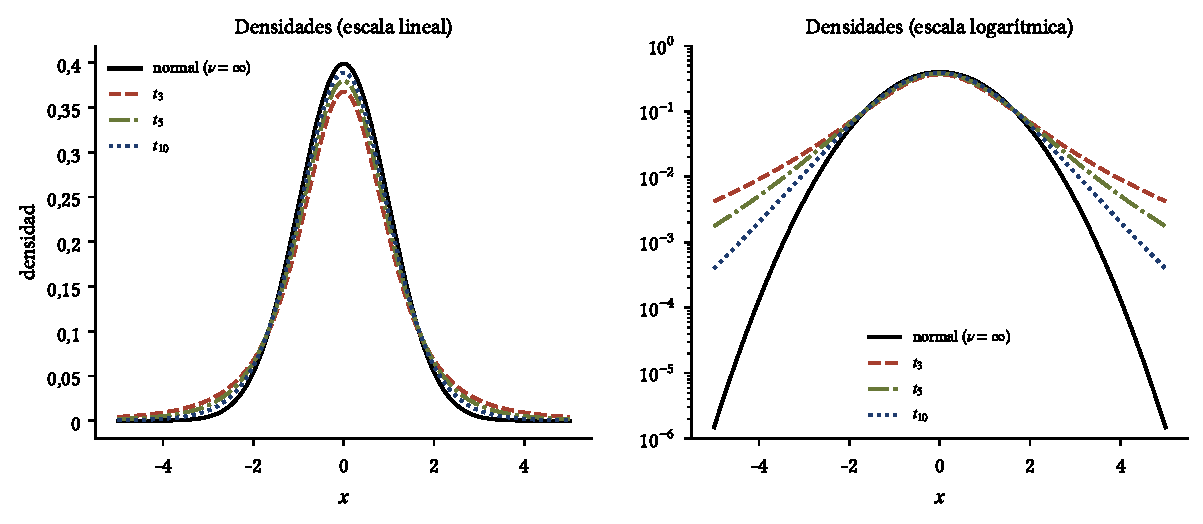
\includegraphics[width=\linewidth]{graficos/cap02_fig_tstudent.pdf}
\caption{Densidades $t$ de Student con $\nu=3,5,10$ y la normal estándar. Izquierda: escala lineal. Derecha: escala logarítmica, donde la normal es una parábola. A cinco unidades del centro, la densidad de la $t_3$ es unas 2\,800 veces la de la normal.}
\label{fig:tstudent}
\end{figure}


\subsection{Colas de tipo Pareto e índice de cola}

Una forma más general de describir colas pesadas es decir que, para pérdidas grandes, la probabilidad de
superar un umbral decae como una potencia y no exponencialmente.

\begin{definicion}[Cola de tipo Pareto]
Una variable $X$ tiene cola derecha de tipo Pareto con \emph{índice de cola} $\alpha>0$ si, para valores
grandes de $x$, $P(X>x)\approx C\,x^{-\alpha}$. Cuanto menor es $\alpha$, más pesada es la cola. La normal
tiene colas que decaen como $e^{-x^2/2}$, más rápido que cualquier potencia: su índice es ``infinito''.
\end{definicion}

\begin{proposicion}[Momentos e índice de cola]\label{prop:momentos_cola}
Si $X\ge u>0$ tiene distribución de Pareto, $P(X>x)=(x/u)^{-\alpha}$ para $x\ge u$, entonces $\E X^k$ es
finito si y solo si $k<\alpha$.
\end{proposicion}

\begin{proof}
La densidad se obtiene derivando la función de distribución:
\begin{align*}
  f(x) &= -\frac{d}{dx}\Bigl(\frac{x}{u}\Bigr)^{-\alpha}\\
       &= \alpha\,u^{\alpha}x^{-\alpha-1}, \qquad x\ge u .
\end{align*}
Entonces
\begin{align*}
  \E[X^k] &= \int_u^\infty x^k\,\alpha u^{\alpha}x^{-\alpha-1}\,dx\\
          &= \alpha u^{\alpha}\int_u^\infty x^{k-\alpha-1}\,dx .
\end{align*}
La integral converge si y solo si $k-\alpha-1<-1$, es decir, $k<\alpha$. En ese caso
\begin{align*}
  \E[X^k] &= \alpha u^{\alpha}\Bigl[\frac{x^{k-\alpha}}{k-\alpha}\Bigr]_u^\infty\\
          &= \alpha u^{\alpha}\cdot\frac{0-u^{k-\alpha}}{k-\alpha}\\
          &= \frac{\alpha\,u^{k}}{\alpha-k}. && \qedhere
\end{align*}
\end{proof}

La consecuencia práctica es fuerte: si los rendimientos tienen índice de cola $\alpha$ entre 2 y 4, la
varianza existe pero la curtosis \emph{poblacional} es infinita. La curtosis muestral sigue siendo un
número finito, pero no converge a nada cuando crece la muestra: su valor depende de cuáles eventos
extremos cayeron en la muestra. Lo comprobaremos con el Brent. La Figura~\ref{fig:pareto} muestra por qué el índice de cola se lee como una pendiente: en escala logarítmica doble, $\ln P(X>x)=\ln C-\alpha\ln x$ es una recta de pendiente $-\alpha$.
\begin{figure}[ht]
\centering
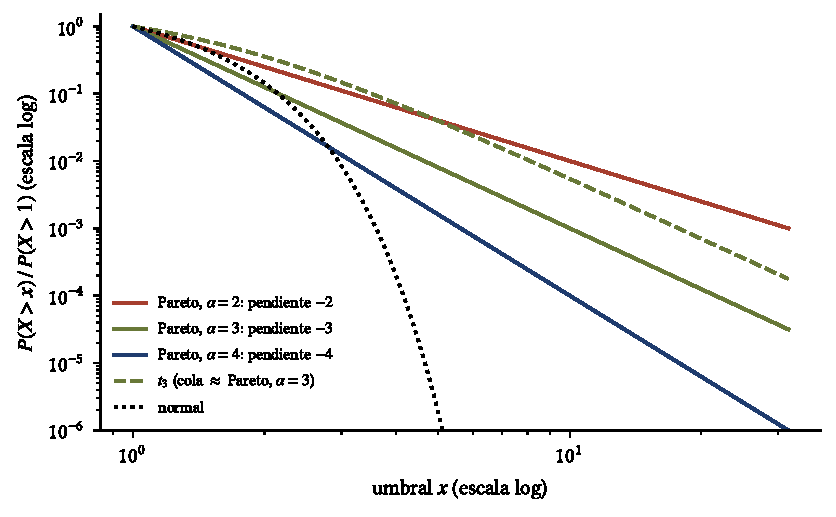
\includegraphics[width=0.75\linewidth]{graficos/cap02_fig_pareto.pdf}
\caption{Probabilidad de superar un umbral, en escala logarítmica doble. Las colas de Pareto son rectas de pendiente $-\alpha$; la $t_3$ termina comportándose como una Pareto con $\alpha=3$; la normal se desploma: su cola decae más rápido que cualquier potencia.}
\label{fig:pareto}
\end{figure}


\begin{proposicion}[Estimador de Hill]\label{prop:hill}
Sean $X_{(1)}\ge X_{(2)}\ge\cdots$ las observaciones ordenadas de mayor a menor. Si las $k$ mayores
observaciones, condicionadas a superar $u=X_{(k+1)}$, siguen una distribución de Pareto con índice
$\alpha$, el estimador de máxima verosimilitud de $\alpha$ es el \emph{estimador de Hill}
\[
  \hat\alpha=\left[\frac1k\sum_{i=1}^k\ln\frac{X_{(i)}}{X_{(k+1)}}\right]^{-1},
\]
con varianza asintótica $\alpha^2/k$.
\end{proposicion}

\begin{proof}
Si $X$ es Pareto por encima de $u$, la variable $Y=\ln(X/u)$ cumple
\begin{align*}
  P(Y>y) &= P\bigl(\ln(X/u)>y\bigr)\\
         &= P\bigl(X>u\,e^{y}\bigr)\\
         &= \Bigl(\frac{u\,e^{y}}{u}\Bigr)^{-\alpha}\\
         &= e^{-\alpha y}:
\end{align*}
es exponencial con tasa $\alpha$ y densidad $\alpha e^{-\alpha y}$. La log-verosimilitud de $k$
observaciones $y_1,\dots,y_k$ y sus derivadas son
\begin{align*}
  \ell(\alpha)   &= \sum_{i=1}^k\ln\bigl(\alpha\,e^{-\alpha y_i}\bigr)\\
                 &= k\ln\alpha-\alpha\sum_{i=1}^ky_i,\\
  \ell'(\alpha)  &= \frac{k}{\alpha}-\sum_{i=1}^ky_i,\\
  \ell''(\alpha) &= -\frac{k}{\alpha^2}.
\end{align*}
Igualando la primera derivada a cero, con $y_i=\ln\bigl(X_{(i)}/X_{(k+1)}\bigr)$:
\begin{align*}
  \frac{k}{\hat\alpha} &= \sum_{i=1}^ky_i\\
  \hat\alpha &= \Bigl[\frac1k\sum_{i=1}^k\ln\frac{X_{(i)}}{X_{(k+1)}}\Bigr]^{-1}.
\end{align*}
La información de Fisher es $-\ell''(\alpha)=k/\alpha^2$, y la varianza asintótica del estimador de máxima
verosimilitud es su inversa:
\begin{align*}
  \Var(\hat\alpha) &\approx \Bigl(\frac{k}{\alpha^2}\Bigr)^{-1}\\
                   &= \frac{\alpha^2}{k}. && \qedhere
\end{align*}
\end{proof}

\begin{observacion}
La elección de $k$ es un compromiso: con $k$ pequeño el estimador usa solo la cola y tiene poco sesgo
pero mucha varianza; con $k$ grande gana precisión pero incluye observaciones donde la aproximación de
Pareto ya no es válida. Por eso se examina $\hat\alpha$ para muchos valores de $k$ (gráfico de Hill) y se
buscan zonas estables.
\end{observacion}

% ---------------------------------------------------------------------
\section{Autocorrelación y dependencia}\label{sec:acf}
% ---------------------------------------------------------------------

\begin{definicion}[Autocorrelación muestral]
La autocorrelación muestral de orden $j$ es
\[
  \hat\rho_j=\frac{\sum_{t=j+1}^T(r_t-\bar r)(r_{t-j}-\bar r)}{\sum_{t=1}^T(r_t-\bar r)^2}.
\]
\end{definicion}

\begin{teorema}[Bartlett]\label{teo:bartlett}
Si $r_t$ es i.i.d. con varianza finita, para cada $m$ fijo el vector
$\sqrt T(\hat\rho_1,\dots,\hat\rho_m)$ converge a una normal con media cero y matriz de covarianzas
identidad. En particular, $\pm1{,}96/\sqrt T$ es una banda de aceptación aproximada al 95\,\% para cada
$\hat\rho_j$, y el estadístico de \emph{Ljung-Box}
\[
  Q(m)=T(T+2)\sum_{j=1}^m\frac{\hat\rho_j^2}{T-j}
\]
converge a una $\chi^2_m$.
\end{teorema}

La demostración usa el teorema central del límite para martingalas y puede consultarse en Brockwell y
Davis (1991, cap.~7). Lo importante aquí es el supuesto: \emph{independencia}, no solo ausencia de
correlación. La siguiente proposición muestra por qué esa diferencia es crucial en finanzas.

\begin{proposicion}[Sin correlación no significa independencia]\label{prop:mds}
Sea $r_t=\sigma_t\varepsilon_t$, donde $\varepsilon_t$ es i.i.d. con media 0 y varianza 1, independiente
de la información pasada $\mathcal F_{t-1}$, y $\sigma_t>0$ depende solo de $\mathcal F_{t-1}$. Entonces:
\begin{enumerate}[label=(\alph*)]
  \item $\Cov(r_t,r_{t-j})=0$ para todo $j\ge1$;
  \item si $\sigma_t^2=\omega+a\,r_{t-1}^2$ con $\omega>0$, $0<a$ y cuarto momento finito, entonces
        $\Cov(r_t^2,r_{t-1}^2)=a\Var(r_{t-1}^2)>0$.
\end{enumerate}
\end{proposicion}

\begin{proof}
(a) Como $\sigma_t$ se conoce en $t-1$ y $\varepsilon_t$ es independiente del pasado,
\begin{align*}
  \E[r_t\mid\mathcal F_{t-1}] &= \E[\sigma_t\varepsilon_t\mid\mathcal F_{t-1}]\\
                              &= \sigma_t\,\E[\varepsilon_t]\\
                              &= 0 .
\end{align*}
Por la ley de esperanzas iteradas, $\E r_t=0$, y como $r_{t-j}$ se conoce en $t-1$:
\begin{align*}
  \Cov(r_t,r_{t-j}) &= \E[r_t\,r_{t-j}]\\
                    &= \E\bigl[\E(r_t\,r_{t-j}\mid\mathcal F_{t-1})\bigr]\\
                    &= \E\bigl[r_{t-j}\,\E(r_t\mid\mathcal F_{t-1})\bigr]\\
                    &= \E[r_{t-j}\cdot0]\\
                    &= 0 .
\end{align*}

(b) Ahora la varianza condicional depende del pasado:
\begin{align*}
  \E[r_t^2\mid\mathcal F_{t-1}] &= \sigma_t^2\,\E[\varepsilon_t^2]\\
                                &= \omega+a\,r_{t-1}^2 .
\end{align*}
Por esperanzas iteradas:
\begin{align*}
  \Cov(r_t^2,r_{t-1}^2)
    &= \E\bigl[r_t^2\,r_{t-1}^2\bigr]-\E\bigl[r_t^2\bigr]\,\E\bigl[r_{t-1}^2\bigr]\\
    &= \E\bigl[r_{t-1}^2\,\E(r_t^2\mid\mathcal F_{t-1})\bigr]
       -\E\bigl[\E(r_t^2\mid\mathcal F_{t-1})\bigr]\,\E\bigl[r_{t-1}^2\bigr]\\
    &= \Cov\bigl(\omega+a\,r_{t-1}^2,\ r_{t-1}^2\bigr)\\
    &= a\,\Var\bigl(r_{t-1}^2\bigr)\\
    &> 0 . && \qedhere
\end{align*}
\end{proof}

El modelo del inciso (b) es el ARCH(1) de Engle (1982), que estudiaremos en el Capítulo~8. La
proposición dice que un mercado puede ser imprevisible en la \emph{dirección} de los precios
(rendimientos sin autocorrelación) y, a la vez, muy previsible en la \emph{magnitud} de los movimientos
(cuadrados autocorrelacionados). Esa es la forma matemática del \emph{agrupamiento de volatilidad}: a
períodos agitados les siguen períodos agitados. La Figura~\ref{fig:arch} lo muestra con una simulación.
\begin{figure}[ht]
\centering
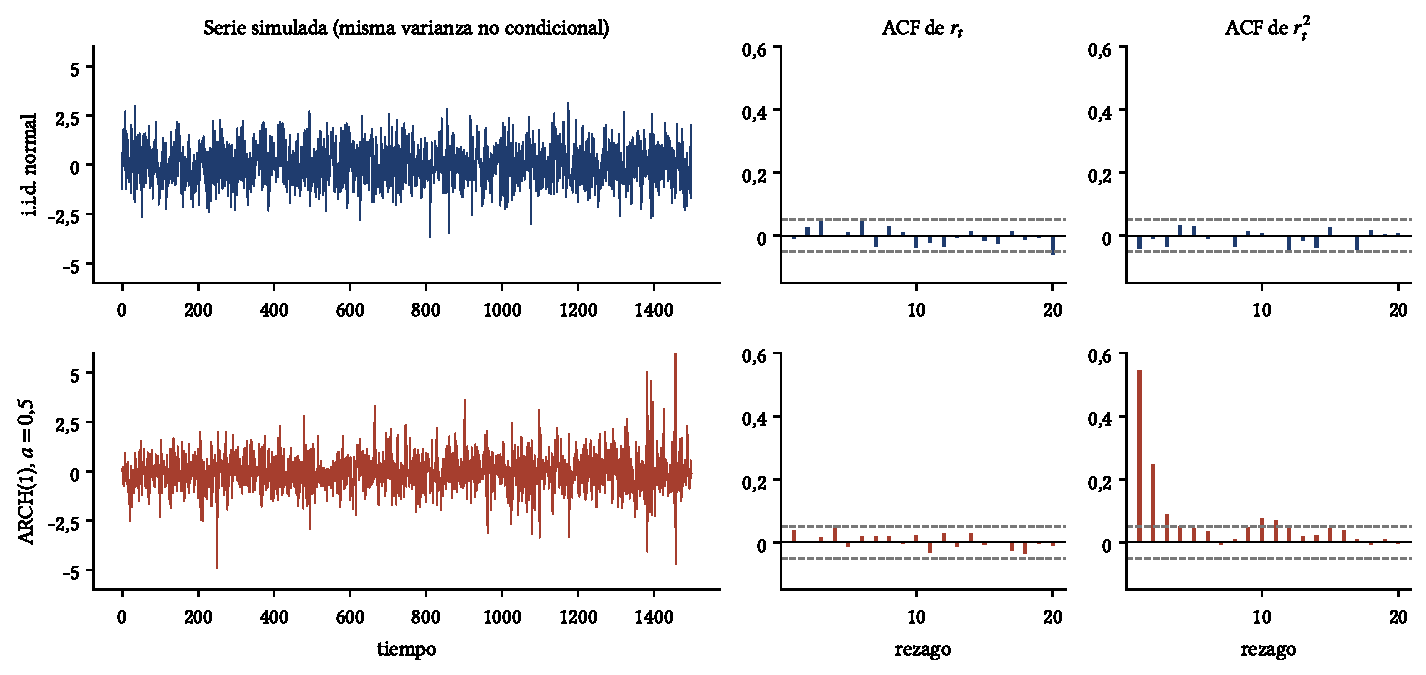
\includegraphics[width=\linewidth]{graficos/cap02_fig_arch.pdf}
\caption{Ruido i.i.d. normal (arriba) frente a un ARCH(1) con $\omega=0{,}5$ y $a=0{,}5$ (abajo), ambos con varianza no condicional 1. Ninguno tiene autocorrelación en $r_t$ (centro), pero solo el ARCH tiene autocorrelación en $r_t^2$ (derecha), y su trayectoria muestra rachas de calma y de turbulencia.}
\label{fig:arch}
\end{figure}


\begin{observacion}[Las bandas de Bartlett con heterocedasticidad]
Si los rendimientos siguen un proceso como el de la Proposición~\ref{prop:mds}, $\hat\rho_j$ sigue
siendo consistente para cero, pero su varianza ya no es $1/T$, sino aproximadamente
$\E[r_t^2r_{t-j}^2]/(T\,\sigma^4)$, que es mayor. Las bandas $\pm1{,}96/\sqrt T$ y la prueba de
Ljung-Box \emph{rechazan demasiado}: detectan autocorrelación donde solo hay volatilidad cambiante. En el
Capítulo~4 corregiremos este problema con errores estándar robustos.
\end{observacion}

% ---------------------------------------------------------------------
\section{Agregación temporal}
% ---------------------------------------------------------------------

Por la Proposición~\ref{prop:aditiva}, el rendimiento logarítmico de $h$ días es la suma de $h$
rendimientos diarios. Si estos tienen varianza finita y dependencia débil, el teorema central del límite
sugiere que la suma se acerca a una normal a medida que $h$ crece: la curtosis de los rendimientos
semanales, mensuales y trimestrales debería ir bajando hacia 3. Este fenómeno se llama
\emph{gaussianidad agregativa}. El índice de cola es la condición clave: si $\alpha>2$, la varianza
existe y el teorema central del límite aplica; si $\alpha<2$, las sumas no se vuelven normales nunca.
La velocidad de convergencia, sin embargo, puede ser lenta, y en muestras finitas unos pocos eventos
extremos pueden dominar los momentos de los rendimientos agregados.

% ---------------------------------------------------------------------
\section{Datos promediados: el efecto de Working}\label{sec:working}
% ---------------------------------------------------------------------

Muchas series publicadas no son precios observados en un instante, sino promedios del período: el
S\&P 500 mensual de Shiller es el promedio de los cierres diarios de cada mes; el tipo de cambio
\emph{promedio} mensual del BCRP también lo es. Working (1960) mostró que promediar crea autocorrelación
donde no la hay.

\begin{proposicion}[Working, 1960]\label{prop:working}
Sea $W(s)$ un movimiento browniano estándar (versión continua de un paseo aleatorio) y
$A_k=\int_{k-1}^{k}W(s)\,ds$ el promedio del período $k$. Los cambios $\Delta A_k=A_k-A_{k-1}$ cumplen
\[
  \Var(\Delta A_k)=\tfrac23,\qquad \Cov(\Delta A_k,\Delta A_{k-1})=\tfrac16,\qquad
  \operatorname{Corr}(\Delta A_k,\Delta A_{k-1})=\tfrac14,
\]
y la autocorrelación de orden $j\ge2$ es cero.
\end{proposicion}

\begin{proof}
Escribimos el cambio de los promedios como una integral de incrementos:
\begin{align*}
  \Delta A_k &= \int_0^1W(k-1+s)\,ds-\int_0^1W(k-2+s)\,ds\\
             &= \int_0^1\bigl[W(k-1+s)-W(k-2+s)\bigr]ds\\
             &= \int_0^1I(s)\,ds,
\end{align*}
donde $I(s)$ es el incremento del browniano en el intervalo $(k-2+s,\,k-1+s]$, de longitud 1. Para un
browniano, la covarianza de dos incrementos es la longitud de la intersección de sus intervalos.

\emph{Varianza.} Los intervalos de $I(s)$ e $I(v)$ se intersecan en una longitud $1-|s-v|$:
\begin{align*}
  \Var(\Delta A_k) &= \int_0^1\!\!\int_0^1\Cov\bigl(I(s),I(v)\bigr)\,ds\,dv\\
                   &= \int_0^1\!\!\int_0^1(1-|s-v|)\,ds\,dv\\
                   &= 1-\int_0^1\!\!\int_0^1|s-v|\,ds\,dv\\
                   &= 1-\tfrac13\\
                   &= \tfrac23 .
\end{align*}
La integral de $|s-v|$ se calcula por simetría, separando las zonas $s<v$ y $s>v$:
\begin{align*}
  \int_0^1\!\!\int_0^1|s-v|\,ds\,dv &= 2\int_0^1\!\!\int_0^v(v-s)\,ds\,dv\\
                                    &= 2\int_0^1\frac{v^2}{2}\,dv\\
                                    &= \int_0^1v^2\,dv\\
                                    &= \tfrac13 .
\end{align*}

\emph{Covarianza de orden 1.} $\Delta A_{k-1}=\int_0^1J(v)\,dv$, con $J(v)$ el incremento en
$(k-3+v,\,k-2+v]$. Ese intervalo y el de $I(s)$ se intersecan en $(k-2+s,\,k-2+v]$, de longitud
$\max(0,v-s)$:
\begin{align*}
  \Cov(\Delta A_k,\Delta A_{k-1}) &= \int_0^1\!\!\int_0^1\max(0,v-s)\,ds\,dv\\
                                  &= \int_0^1\!\!\int_0^v(v-s)\,ds\,dv\\
                                  &= \int_0^1\frac{v^2}{2}\,dv\\
                                  &= \tfrac16 .
\end{align*}
Por tanto,
\begin{align*}
  \operatorname{Corr}(\Delta A_k,\Delta A_{k-1}) &= \frac{1/6}{2/3}\\
                                                 &= \frac14 .
\end{align*}
Para $j\ge2$, los intervalos de $I(s)$ y del incremento de $\Delta A_{k-j}$ no se intersecan, y la
covarianza es cero.
\end{proof}

\begin{observacion}
Con $n$ observaciones discretas por período, Working obtuvo
$\rho_1=(n^2-1)/[2(2n^2+1)]$, que vale $0{,}2492$ para $n=21$ días hábiles por mes y tiende a $1/4$
cuando $n\to\infty$. Un analista que estime un modelo ARMA sobre los rendimientos del S\&P 500 de Shiller
``descubrirá'' una autocorrelación de 0,25 que no dice nada sobre la eficiencia del mercado: es un
artefacto de cómo se construyeron los datos. Siempre hay que saber si una serie es de fin de período o
de promedio del período.
\end{observacion}

% ---------------------------------------------------------------------
\section{Catálogo de hechos estilizados}
% ---------------------------------------------------------------------

Siguiendo a Cont (2001), resumimos los hechos que documentaremos y que los modelos posteriores deben
reproducir.

\begin{table}[ht]
\centering\small
\begin{tabularx}{\linewidth}{@{}>{\raggedright\arraybackslash}p{3.6cm}X>{\raggedright\arraybackslash}p{2.6cm}@{}}
\toprule
Hecho & Descripción & Modelo que lo captura \\
\midrule
Colas pesadas & Curtosis muy superior a 3; índice de cola entre 2 y 5. & $t$ de Student, valores extremos (Cap.~9, 13) \\
Asimetría de pérdidas & Las caídas extremas son mayores que las subidas extremas. & GARCH asimétricos (Cap.~9) \\
Ausencia de autocorrelación lineal & $\hat\rho_j$ de los rendimientos cercanos a cero, salvo en frecuencias muy altas o datos promediados. & Eficiencia de mercado (Cap.~7) \\
Agrupamiento de volatilidad & Autocorrelación positiva y persistente de $r_t^2$ y $|r_t|$. & ARCH/GARCH (Cap.~8) \\
Memoria larga de la volatilidad & La autocorrelación de $|r_t|$ decae muy lentamente. & GARCH integrados, modelos de componentes \\
Gaussianidad agregativa & La distribución se acerca a la normal al aumentar el horizonte. & Teorema central del límite \\
\bottomrule
\end{tabularx}
\caption{Hechos estilizados de los rendimientos financieros.}
\label{tab:hechos}
\end{table}

% ---------------------------------------------------------------------
\section{Ejercicios resueltos}
% ---------------------------------------------------------------------

\begin{ejresuelto}{¿Son normales los rendimientos diarios del petróleo Brent?}\label{ej:brentnormal}
\enunciado Con los precios spot diarios del Brent (EIA, 1987--2026): (a) calcule la media, la desviación
estándar, la asimetría, la curtosis y el estadístico de Jarque-Bera de los rendimientos logarítmicos;
(b) identifique los días más extremos; (c) evalúe la sensibilidad de los momentos a los dos días de abril
de 2020; (d) compare la frecuencia de movimientos mayores a cuatro desviaciones estándar con la que
predice la normal.

\solucion
\paso{Paso 1. Momentos.} Con $T=9\,121$ rendimientos, la media diaria es $0{,}000192$ (unos
$0{,}019$\,\% por día) y la desviación estándar $\hat\sigma=0{,}0270$. La asimetría es $\hat S=-1{,}49$ y
la curtosis $\hat K=55{,}97$: casi diecinueve veces la de una normal.

\paso{Paso 2. Jarque-Bera.} Sustituimos en la fórmula del Teorema~\ref{teo:jb}:
\begin{align*}
  JB &= \frac{T}{6}\Bigl[\hat S^2+\frac{(\hat K-3)^2}{4}\Bigr]\\
     &= \frac{9\,121}{6}\Bigl[(-1{,}4937)^2+\frac{(55{,}966-3)^2}{4}\Bigr]\\
     &= 1\,520{,}17\times\Bigl[2{,}2311+\frac{2\,805{,}40}{4}\Bigr]\\
     &= 1\,520{,}17\times\bigl[2{,}2311+701{,}35\bigr]\\
     &= 1\,520{,}17\times703{,}58\\
     &\approx 1{,}0696\times10^{6}.
\end{align*}
Con todos los decimales se obtiene $1{,}0695\times10^{6}$, el valor de la salida. El valor crítico de la
$\chi^2_2$ al 5\,\% es $5{,}99$: la normalidad se rechaza de forma abrumadora. Casi todo el estadístico
proviene de la curtosis; el término de asimetría aporta solo
\begin{align*}
  \frac{T}{6}\,\hat S^2 &= 1\,520{,}17\times2{,}2311\\
                        &\approx 3\,392 .
\end{align*}

\paso{Paso 3. Días extremos.} Los cinco mayores movimientos son el 21 y el 22 de abril de 2020
($-64{,}4$\,\% y $+41{,}2$\,\%), el 17 de enero de 1991 ($-36{,}1$\,\%, inicio de la operación Tormenta
del Desierto en la Guerra del Golfo), y el 2 y el 31 de marzo de 2020. Cuatro de los cinco ocurren en
el primer semestre de 2020.

\paso{Paso 4. Sensibilidad.} Al quitar solo dos días de 9\,121 (el 0,02\,\% de la muestra), la
curtosis cae de 55,97 a 17,79 y la asimetría de $-1{,}49$ a $-0{,}46$. Un estimador que cambia tanto al
eliminar dos datos no está midiendo una propiedad estable de la distribución. Es la señal empírica de
que el cuarto momento poblacional quizá no exista, lo que verificaremos en el Ejercicio~\ref{ej:hill}.

\paso{Paso 5. Eventos de cuatro sigmas.} Comparamos el número de días con $|z_t|>4$ observado y el que
predice la normal:
\begin{align*}
  \text{días observados}  &= 0{,}005591\times9\,121\\
                          &\approx 51,\\
  \text{días esperados}   &= 2\,\Phi(-4)\times9\,121\\
                          &= 6{,}334\times10^{-5}\times9\,121\\
                          &\approx 0{,}58,\\
  \text{cociente}         &= \frac{0{,}005591}{6{,}334\times10^{-5}}\\
                          &\approx 88 .
\end{align*}
Los movimientos extremos son 88 veces más frecuentes de lo que supone la normal.

\codigoweb{cap02_ej01}
\salidaR{cap02_ej01_R.txt}
\lectura{cap02_ej01}

\RvsPy R no trae funciones de asimetría y curtosis en su instalación base, así que las programamos
directamente desde la definición; Python las toma de \texttt{scipy.stats}. Hay que fijar en Python
\texttt{fisher=False} para obtener la curtosis (y no el exceso de curtosis) y \texttt{ddof=0} en la
desviación estándar para que coincida con $\sqrt{m_2}$. Con esas precauciones, ambas salidas coinciden
en todas las cifras.

\begin{figure}[ht]
\centering
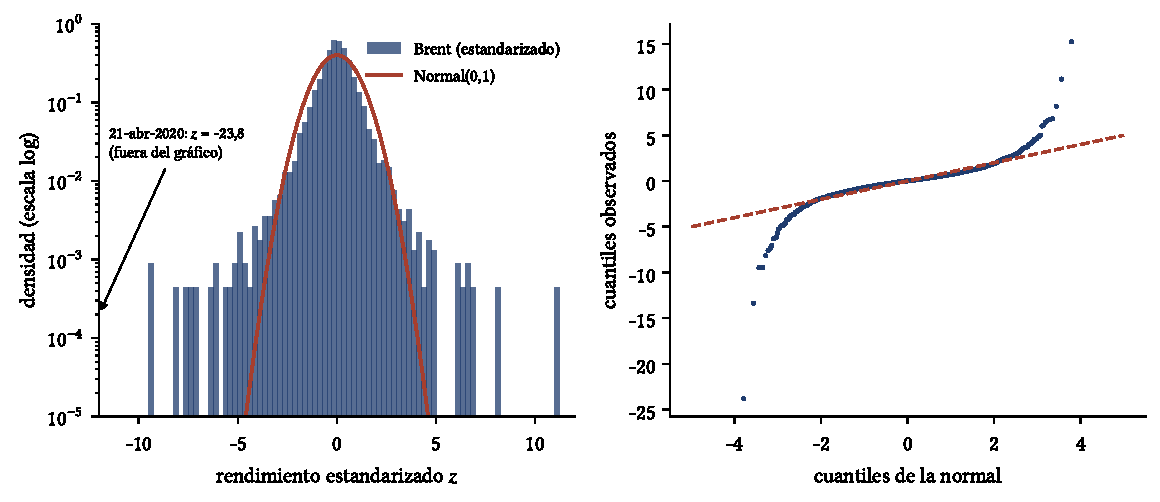
\includegraphics[width=\linewidth]{graficos/cap02_fig_normalidad.pdf}
\caption{Rendimientos diarios estandarizados del Brent, 1987--2026. Izquierda: histograma en escala
logarítmica frente a la densidad normal; la normal es una parábola en esta escala, y los datos tienen
un pico más alto y colas mucho más gruesas. Derecha: gráfico cuantil-cuantil; los puntos se separan de
la recta en ambos extremos, con más fuerza en las pérdidas.}
\label{fig:normalidad}
\end{figure}

\begin{conclusion}
Los rendimientos diarios del Brent no son normales: tienen colas extremadamente pesadas y asimetría
negativa. Un modelo de riesgo basado en la normal subestimaría la frecuencia de movimientos extremos
en un factor cercano a 90. Además, la curtosis muestral es inestable y depende de unos pocos días, por
lo que no debe reportarse sin un análisis de sensibilidad.
\end{conclusion}
\end{ejresuelto}

\begin{ejresuelto}{Rendimientos impredecibles, volatilidad predecible}\label{ej:acf}
\enunciado Con los rendimientos diarios del Brent: (a) calcule las autocorrelaciones de orden 1 a 10 de
$r_t$, $r_t^2$ y $|r_t|$; (b) aplique la prueba de Ljung-Box con $m=10$ y $m=20$; (c) interprete los
resultados a la luz de la Proposición~\ref{prop:mds}.

\solucion
\paso{Paso 1. Banda de referencia.} Con $T=9\,121$, la banda de Bartlett al 95\,\% es
\begin{align*}
  \pm\frac{1{,}96}{\sqrt T} &= \pm\frac{1{,}96}{\sqrt{9\,121}}\\
                            &= \pm\frac{1{,}96}{95{,}50}\\
                            &= \pm0{,}0205 .
\end{align*}

\paso{Paso 2. Rendimientos.} Las diez autocorrelaciones de $r_t$ están entre $-0{,}028$ y $0{,}021$;
la de primer orden es $-0{,}003$. Tres de ellas rozan la banda (rezagos 2, 8 y 10), pero ninguna tiene
importancia económica: una autocorrelación de 0,02 explica el 0,04\,\% de la varianza del día siguiente.

\paso{Paso 3. Cuadrados y valores absolutos.} La autocorrelación de primer orden de $r_t^2$ es $0{,}33$,
dieciséis veces la banda, y la de $|r_t|$ es $0{,}26$. Todas las autocorrelaciones de $|r_t|$ hasta el
rezago 10 están entre 0,18 y 0,26, y la Figura~\ref{fig:acf} muestra que siguen siendo positivas y
significativas más allá del rezago 100: la volatilidad tiene una memoria muy larga.

\paso{Paso 4. Ljung-Box.} Para $|r_t|$, $Q(10)=4\,170{,}8$ y para $r_t^2$, $Q(10)=1\,721{,}3$, frente a un
valor crítico de $\chi^2_{10}$ al 5\,\% de $18{,}3$: rechazo abrumador. Para $r_t$, $Q(10)=25{,}74$
($p=0{,}0041$) también rechaza. Este último resultado debe leerse con cuidado: por la observación que
sigue a la Proposición~\ref{prop:mds}, la prueba de Ljung-Box rechaza en exceso cuando la volatilidad
cambia en el tiempo, que es justamente lo que muestran los pasos~3 y~4. El rechazo para $r_t$ es
compatible con autocorrelaciones verdaderas nulas y volatilidad cambiante; en el Capítulo~4 lo
verificaremos con una versión robusta de la prueba.

\codigoweb{cap02_ej02}
\salidaR{cap02_ej02_R.txt}
\lectura{cap02_ej02}

\RvsPy \texttt{acf()} y \texttt{Box.test()} pertenecen a la instalación base de R; en Python usamos
\texttt{statsmodels}. Las dos funciones de autocorrelación usan el mismo denominador $\sum(r_t-\bar r)^2$
para todos los rezagos, por lo que los valores coinciden. Para el $p$-valor en R calculamos la cola
superior con \texttt{pchisq(..., lower.tail = FALSE)}: la salida por defecto de \texttt{Box.test()}
calcula $1-F(Q)$ y redondea a cero los $p$-valores muy pequeños.

\begin{figure}[ht]
\centering
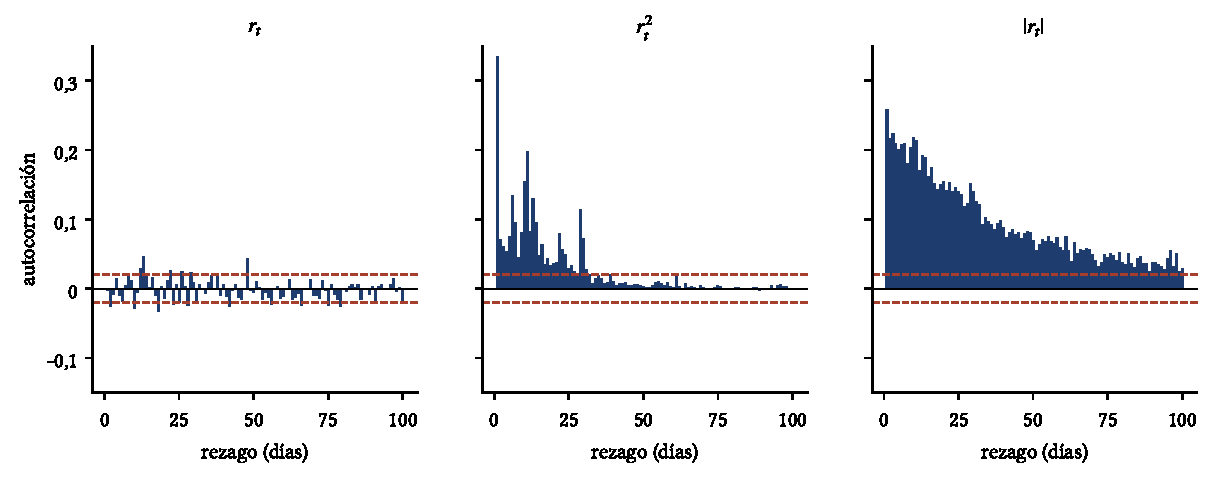
\includegraphics[width=\linewidth]{graficos/cap02_fig_acf.pdf}
\caption{Autocorrelaciones del Brent hasta el rezago 100, con la banda de Bartlett al 95\,\% (líneas
discontinuas). Los rendimientos casi no tienen autocorrelación; sus cuadrados y, sobre todo, sus valores
absolutos tienen autocorrelaciones positivas que decaen muy lentamente.}
\label{fig:acf}
\end{figure}

\begin{conclusion}
El Brent ilustra la Proposición~\ref{prop:mds}: la dirección del precio de mañana es prácticamente
impredecible a partir de los rendimientos pasados, pero su volatilidad es altamente predecible. Este es
el hecho estilizado que motiva los modelos ARCH y GARCH.
\end{conclusion}
\end{ejresuelto}

\begin{ejresuelto}{¿Se vuelven normales los rendimientos al agregarlos?}\label{ej:agregacion}
\enunciado Agregue los rendimientos diarios del Brent en bloques sin traslape de $h=1,5,21,63$ y $126$
días de negociación (aproximadamente día, semana, mes, trimestre y semestre). Para cada horizonte calcule
la desviación estándar, la asimetría, la curtosis y el $p$-valor de Jarque-Bera. ¿Se cumple la
gaussianidad agregativa? ¿Se cumple la regla de la raíz del tiempo?

\solucion
\paso{Paso 1. Tendencia general.} La curtosis cae de 55,97 ($h=1$) a 14,81 ($h=5$), 4,93 ($h=63$) y
3,84 ($h=126$). Con bloques semestrales, Jarque-Bera ya no rechaza la normalidad ($p=0{,}344$), aunque
con solo 72 observaciones la prueba tiene poca potencia.

\paso{Paso 2. Una excepción instructiva.} Con $h=21$ la curtosis \emph{sube} a 24,93. La razón es que,
con 434 observaciones mensuales, un único mes extremo (marzo-abril de 2020) pesa muchísimo en el cuarto
momento. La Figura~\ref{fig:agregacion} muestra que el pico en $h=21$ persiste incluso sin el 21 y el
22 de abril de 2020: no lo producen dos días, sino un período completo de crisis. La convergencia a la
normal existe, pero es lenta y errática cuando las colas son tan pesadas como las del
Ejercicio~\ref{ej:hill}.

\paso{Paso 3. Raíz del tiempo.} Comparamos el cociente de volatilidades con el que predice la regla:
\begin{align*}
  \frac{\hat\sigma_{21}}{\hat\sigma_{1}} &= \frac{0{,}12807}{0{,}027039}\\
                                          &= 4{,}736,\\
  \sqrt{21}                               &= 4{,}583,\\
  \frac{4{,}736}{4{,}583}                 &= 1{,}033 .
\end{align*}
La volatilidad mensual es un 3,3\,\% mayor de lo que predice la regla de la raíz del tiempo, una
diferencia moderada. Por la Proposición~\ref{prop:agregmom}, apunta a una leve autocorrelación positiva
acumulada en los rendimientos diarios, o simplemente al peso de 2020 en una muestra mensual pequeña.

\codigoweb{cap02_ej03}
\salidaR{cap02_ej03_R.txt}
\lectura{cap02_ej03}

\RvsPy La agregación sin traslape se resuelve igual en ambos lenguajes: se descarta el bloque final
incompleto y se ordenan los datos en una matriz de $h$ filas (R, que llena por columnas) o de $h$
columnas (Python, que llena por filas), sumando luego a lo largo del bloque. Confundir el orden de
llenado es un error frecuente que produce sumas de días no consecutivos.

\begin{figure}[ht]
\centering
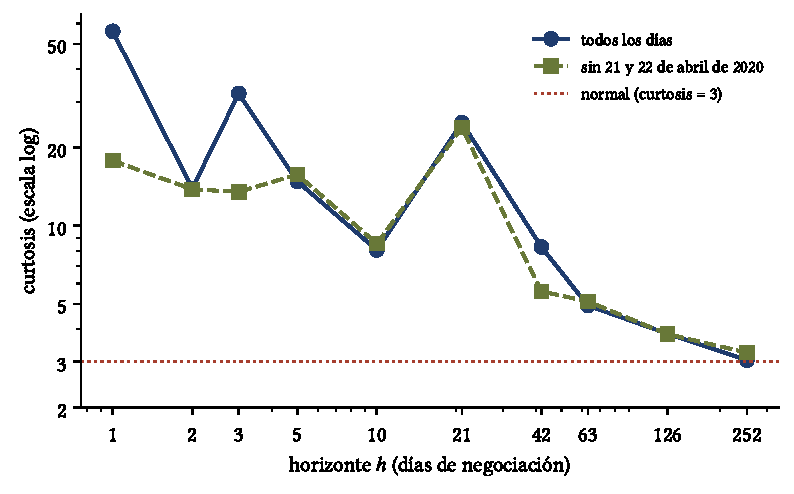
\includegraphics[width=0.8\linewidth]{graficos/cap02_fig_agregacion.pdf}
\caption{Curtosis de los rendimientos del Brent agregados a $h$ días (ambos ejes en escala
logarítmica). La tendencia hacia el valor normal de 3 es clara a partir de $h=42$, pero el camino es
irregular; el pico de $h=21$ refleja la crisis de marzo-abril de 2020.}
\label{fig:agregacion}
\end{figure}

\begin{conclusion}
La gaussianidad agregativa se cumple a horizontes largos, pero no conviene confiar en ella a horizontes
de un mes: la distribución mensual del Brent sigue teniendo colas muy pesadas. Para la gestión de
riesgos a un mes no es seguro suponer normalidad solo porque se trabaja con datos menos frecuentes.
\end{conclusion}
\end{ejresuelto}

\begin{ejresuelto}{Una autocorrelación que no existe: el S\&P 500 mensual de Shiller}\label{ej:working}
\enunciado Con el S\&P 500 mensual de Shiller (1871--2026): (a) calcule las autocorrelaciones de orden 1
a 6 de los cambios logarítmicos mensuales, en la muestra completa y en los tramos 1871--1945 y
1946--2026; (b) compárelas con el valor teórico de Working; (c) concluya si existe evidencia de
predictibilidad en el mercado accionario estadounidense.

\solucion
\paso{Paso 1. Resultado.} La autocorrelación de primer orden es $0{,}274$ en la muestra completa
($T=1\,868$), seis veces la banda de $0{,}045$; Ljung-Box con $m=1$ da $Q=140{,}6$ y $p=1{,}97\times10^{-32}$.
Los rezagos 2 a 6 son pequeños: entre $-0{,}040$ y $0{,}073$.

\paso{Paso 2. Comparación con Working.} El patrón (una autocorrelación cercana a 0,25 en el primer rezago
y casi nada después) es exactamente el de la Proposición~\ref{prop:working}, con valor teórico de
$0{,}2492$ para 21 días hábiles por mes. La Figura~\ref{fig:working} lo confirma con una simulación: un
paseo aleatorio muestreado a fin de mes no muestra autocorrelación, y el mismo paseo promediado dentro de
cada mes muestra una de $0{,}224$ en el primer rezago, muy cerca del valor de los datos.

\paso{Paso 3. Por tramos.} En 1871--1945 la autocorrelación es $0{,}310$ y en 1946--2026, $0{,}213$.
Ambas están cerca de 1/4. Cada estimación tiene un error estándar aproximado de
$1/\sqrt{900}\approx0{,}033$, así que la diferencia de $0{,}097$ entre tramos equivale a unas dos veces su
error estándar ($\approx0{,}047$): una diferencia marginal que no conviene interpretar sin más análisis.

\codigoweb{cap02_ej04}
\salidaR{cap02_ej04_R.txt}
\lectura{cap02_ej04}

\RvsPy El tratamiento de las fechas difiere: en R se filtra con comparaciones lógicas sobre un vector de
clase \texttt{Date}; en Python, la serie indexada por fechas de \texttt{pandas} permite cortes como
\texttt{r[:"1945-12-01"]}, que incluyen ambos extremos. Los resultados coinciden.

\begin{figure}[ht]
\centering
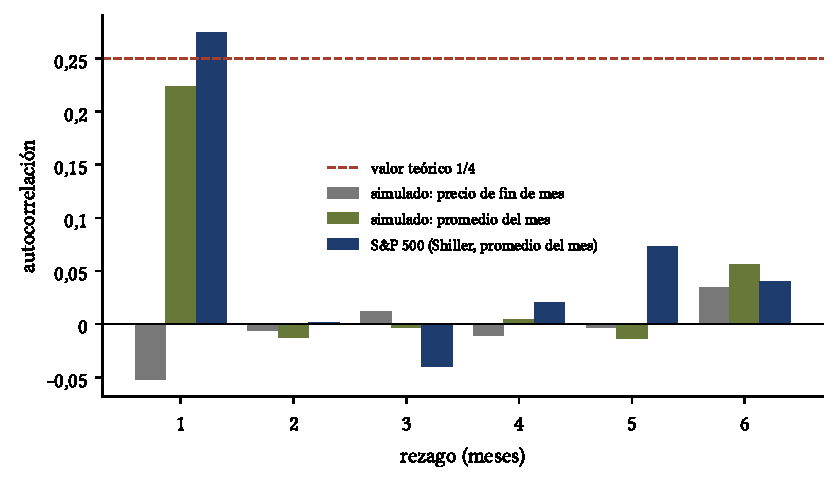
\includegraphics[width=0.82\linewidth]{graficos/cap02_fig_working.pdf}
\caption{Autocorrelaciones de rendimientos mensuales. Un paseo aleatorio simulado no tiene
autocorrelación si se toma el precio de fin de mes (gris), pero sí si se toma el promedio del mes
(verde). El S\&P 500 de Shiller (azul), construido con promedios, reproduce el patrón y se acerca al
valor teórico de 1/4.}
\label{fig:working}
\end{figure}

\begin{conclusion}
La autocorrelación de 0,27 de los rendimientos mensuales de Shiller no es evidencia de que el mercado
estadounidense sea predecible: la explica casi por completo el uso de precios promedio. Antes de
interpretar cualquier autocorrelación, hay que verificar cómo se construyó la serie. La misma advertencia
aplica al tipo de cambio \emph{promedio} mensual que publica el BCRP.
\end{conclusion}
\end{ejresuelto}

\begin{ejresuelto}{¿Qué tan pesadas son las colas del Brent?}\label{ej:hill}
\enunciado Estime el índice de cola del Brent con el estimador de Hill, por separado para las pérdidas
($-r_t$) y para las ganancias ($r_t$), con $k=50,100,200$ y $400$. Construya el gráfico de Hill para
$k$ entre 20 y 900. ¿Existe la varianza? ¿Existe la curtosis?

\solucion
\paso{Paso 1. Estimaciones.} Para las pérdidas, $\hat\alpha$ toma los valores $2{,}52$, $2{,}76$, $2{,}56$
y $2{,}67$; para las ganancias, $2{,}94$, $3{,}30$, $2{,}85$ y $2{,}56$. Los errores estándar
$\hat\alpha/\sqrt k$ van de $0{,}36$ ($k=50$) a $0{,}13$ ($k=400$).

\paso{Paso 2. Intervalos.} Con $k=200$, el intervalo de confianza aproximado al 95\,\% para la cola de
pérdidas es
\begin{align*}
  \hat\alpha\pm1{,}96\,\operatorname{ee}(\hat\alpha) &= 2{,}558\pm1{,}96\times0{,}181\\
                                                     &= 2{,}558\pm0{,}355\\
                                                     &= [2{,}20;\ 2{,}91].
\end{align*}
Está entero por encima de 2 y entero por debajo de 4.

\paso{Paso 3. Interpretación.} Por la Proposición~\ref{prop:momentos_cola}, con $2<\alpha<4$ la varianza
existe pero el cuarto momento no. Esto explica lo que vimos en los ejercicios anteriores: una curtosis
muestral enorme e inestable, que cambia mucho al quitar dos datos (Ejercicio~\ref{ej:brentnormal}) y que
converge lentamente a 3 al agregar (Ejercicio~\ref{ej:agregacion}). La curtosis de 55,97 no es una
``medida'' del riesgo de cola del Brent; el índice de cola sí lo es.

\paso{Paso 4. Asimetría de las colas.} Para $k\le200$ la cola de pérdidas es algo más pesada (menor
$\alpha$) que la de ganancias, en línea con la asimetría negativa; para $k=400$ ambas se igualan.

\codigoweb{cap02_ej05}
\salidaR{cap02_ej05_R.txt}
\lectura{cap02_ej05}

\RvsPy Ambos programas ordenan los datos de mayor a menor (\texttt{sort(..., decreasing = TRUE)} en R y
\texttt{np.sort(...)[::-1]} en Python). Hay que cuidar el índice del umbral: en R, cuya indexación
empieza en 1, el umbral $X_{(k+1)}$ es \texttt{xs[k + 1]}; en Python, que empieza en 0, es
\texttt{xs[k]}. Un error en este índice cambia los resultados sin producir ningún mensaje de error.

\begin{figure}[ht]
\centering
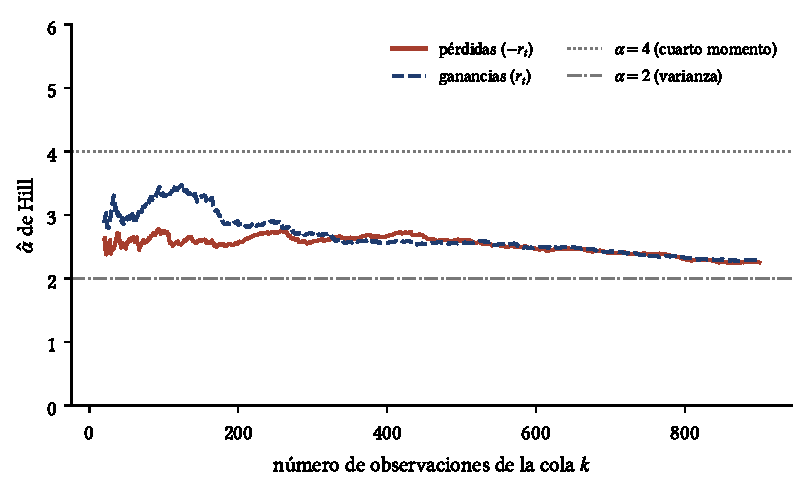
\includegraphics[width=0.82\linewidth]{graficos/cap02_fig_hill.pdf}
\caption{Gráfico de Hill del Brent. Para casi todo el rango de $k$, el índice de cola estimado está entre
2 y 4: la varianza existe, pero el cuarto momento no.}
\label{fig:hill}
\end{figure}

\begin{conclusion}
El índice de cola del Brent está alrededor de 2,5 a 3. La varianza existe, de modo que la volatilidad es
una medida legítima de riesgo, pero el cuarto momento probablemente no, de modo que la curtosis muestral
no debe usarse como medida de riesgo de cola. Para medir riesgos extremos usaremos la teoría de valores
extremos del Capítulo~13.
\end{conclusion}
\end{ejresuelto}

% ---------------------------------------------------------------------
\section{Ejercicios propuestos}
% ---------------------------------------------------------------------

\begin{enumerate}[label=\textbf{\thechapter.\arabic*},leftmargin=*,itemsep=6pt]
  \item Demuestre que $\hat S$ y $\hat K$ no cambian si se reemplaza $r_t$ por $a+br_t$ con $b>0$. ¿Qué
  le ocurre a $\hat S$ si $b<0$? \textit{Respuesta: $\hat S$ cambia de signo y $\hat K$ no cambia.}

  \item Use la Proposición~\ref{prop:curt_t} para hallar los grados de libertad de una $t$ de Student con
  la misma curtosis que el Brent sin los dos días de abril de 2020 ($\hat K=17{,}79$). ¿Es coherente
  con el índice de cola estimado en el Ejercicio~\ref{ej:hill}, sabiendo que el índice de cola de una
  $t_\nu$ es $\nu$? \textit{Respuesta: $\nu=4+6/14{,}79\approx4{,}41$; es mayor que el $\hat\alpha$ de
  Hill, pero del mismo orden.}

  \item Demuestre que, para una Pareto con índice $\alpha>4$ por encima de $u$, la curtosis es
  $K=\dfrac{3(\alpha-2)(3\alpha^2+\alpha+2)}{\alpha(\alpha-3)(\alpha-4)}$ y que tiende a 9 cuando
  $\alpha\to\infty$. \textit{Pista: use los momentos $\E X^k=\alpha u^k/(\alpha-k)$ de la
  Proposición~\ref{prop:momentos_cola}.}

  \item Para el modelo ARCH(1) de la Proposición~\ref{prop:mds}(b) con $\varepsilon_t\sim N(0,1)$, muestre
  que si $3a^2<1$ la curtosis no condicional de $r_t$ es $3(1-a^2)/(1-3a^2)>3$. Concluya que el
  agrupamiento de volatilidad por sí solo genera colas pesadas, aun con innovaciones normales.

  \item Verifique por simulación la fórmula discreta de Working, $\rho_1=(n^2-1)/[2(2n^2+1)]$, para
  $n=5$ y $n=21$. Luego demuéstrela, reemplazando las integrales de la Proposición~\ref{prop:working} por
  sumas. \textit{Respuesta: $0{,}2353$ y $0{,}2492$.}

  \item \emph{(Con datos.)} Con la serie del VIX (\texttt{datos/internacional/vix\_diario.csv}),
  calcule la autocorrelación de los cambios logarítmicos diarios y la del nivel del índice hasta el
  rezago 50. ¿Qué hecho estilizado refleja el nivel del VIX? ¿Por qué sus cambios tienen autocorrelación
  negativa en el primer rezago?

  \item \emph{(Con datos del Capítulo~\ref{cap:rendimientos}.)} Repita los Ejercicios~\ref{ej:brentnormal}
  y~\ref{ej:hill} con el índice S\&P/BVL Perú General y con las acciones de Southern Copper y
  Buenaventura. ¿Tienen las acciones mineras peruanas colas más pesadas que el índice? ¿Por qué cabría
  esperarlo?

  \item \emph{(Con datos del BCRP, investigación.)} Descargue el tipo de cambio interbancario diario y el
  tipo de cambio promedio mensual. Calcule la autocorrelación de primer orden de los cambios mensuales
  con ambas series (para la diaria, tome el último dato de cada mes). ¿Encuentra el efecto de Working?
\end{enumerate}

% ---------------------------------------------------------------------
\section{Resumen de fórmulas}
% ---------------------------------------------------------------------

\begin{table}[H]
\centering\small
\begin{tabular}{@{}ll@{}}
\toprule
Concepto & Fórmula \\
\midrule
Asimetría y curtosis & $\hat S=m_3/m_2^{3/2}$;\quad $\hat K=m_4/m_2^{2}$ \\
Jarque-Bera & $JB=T\bigl[\hat S^2/6+(\hat K-3)^2/24\bigr]\xrightarrow{d}\chi^2_2$ \\
Curtosis de la $t_\nu$ & $K=3+6/(\nu-4)$,\quad $\nu>4$ \\
Momentos de una cola Pareto & $\E X^k<\infty\iff k<\alpha$ \\
Estimador de Hill & $\hat\alpha=\bigl[\frac1k\sum_{i=1}^k\ln(X_{(i)}/X_{(k+1)})\bigr]^{-1}$,\quad $\operatorname{ee}=\hat\alpha/\sqrt k$ \\
Banda de Bartlett & $\pm1{,}96/\sqrt T$ \\
Ljung-Box & $Q(m)=T(T+2)\sum_{j=1}^m\hat\rho_j^2/(T-j)\xrightarrow{d}\chi^2_m$ \\
ARCH(1) & $\Cov(r_t^2,r_{t-1}^2)=a\Var(r_{t-1}^2)$ \\
Efecto de Working & $\rho_1=(n^2-1)/[2(2n^2+1)]\to1/4$ \\
\bottomrule
\end{tabular}
\caption{Fórmulas principales del Capítulo 2.}
\end{table}

\section*{Referencias}
\begin{itemize}[leftmargin=*]
  \item Brockwell, P. J. y Davis, R. A. (1991). \emph{Time Series: Theory and Methods} (2.ª ed.).
        Springer.
  \item Cont, R. (2001). Empirical properties of asset returns: stylized facts and statistical issues.
        \emph{Quantitative Finance}, 1(2), 223--236.
  \item Engle, R. F. (1982). Autoregressive conditional heteroscedasticity with estimates of the variance
        of United Kingdom inflation. \emph{Econometrica}, 50(4), 987--1007.
  \item Hill, B. M. (1975). A simple general approach to inference about the tail of a distribution.
        \emph{The Annals of Statistics}, 3(5), 1163--1174.
  \item Jarque, C. M. y Bera, A. K. (1980). Efficient tests for normality, homoscedasticity and serial
        independence of regression residuals. \emph{Economics Letters}, 6(3), 255--259.
  \item Ljung, G. M. y Box, G. E. P. (1978). On a measure of lack of fit in time series models.
        \emph{Biometrika}, 65(2), 297--303.
  \item Mandelbrot, B. (1963). The variation of certain speculative prices. \emph{The Journal of
        Business}, 36(4), 394--419.
  \item Shiller, R. J. Base de datos de precios, dividendos y utilidades del mercado accionario de
        EE.\,UU., replicada en \url{https://github.com/datasets/s-and-p-500}.
  \item U.S. Energy Information Administration. \emph{Europe Brent Spot Price FOB}, replicada en
        \url{https://github.com/datasets/oil-prices}.
  \item Working, H. (1960). Note on the correlation of first differences of averages in a random chain.
        \emph{Econometrica}, 28(4), 916--918.
\end{itemize}
